%%%%%%%%%%%%%%%%%%%%%%%%%%%%%%%%%%%%%%%%%%%%%%%%%%%%%%%%%%%%%%%%%%%%%%%%%%%%%%
%% Angle-Encoded Quantum Kernels for Stroke Risk Stratification
%% Revised manuscript for the International Journal of Quantum Information
%%
%% Every numerical value in this manuscript is reproduced by reproduce_qksp.py
%% and stored in results.json (or, for the feature-importance and McNemar
%% figures, by analysis.py -> analysis.json). See CHANGES.md.
%%%%%%%%%%%%%%%%%%%%%%%%%%%%%%%%%%%%%%%%%%%%%%%%%%%%%%%%%%%%%%%%%%%%%%%%%%%%%%
\documentclass{ws-ijqi}

\begin{document}

\markboth{S. Shinde \& N. Pikle}
         {Angle-Encoded Quantum Kernels for Stroke Risk Stratification}

\title{Angle-Encoded Quantum Kernels for Stroke Risk\\
       Stratification: An Empirical Comparison with\\
       Classical Kernel Methods}

\author{Snehal Shinde}
\address{Department of Computer Science and Engineering,\\
Indian Institute of Information Technology, Nagpur,\\
Maharashtra 441108, India\\
ssnehalbshinde@gmail.com}

\author{Nileshchandra Pikle}
\address{Department of Computer Science and Engineering,\\
Indian Institute of Information Technology, Nagpur,\\
Maharashtra 441108, India\\
nilesh.pikle@gmail.com}

\maketitle

\begin{history}
\received{Day Month Year}
\revised{Day Month Year}
\accepted{Day Month Year}
\published{Day Month Year}
\end{history}

\begin{abstract}
Early stroke risk stratification supports preventive intervention, and quantum
kernel methods have been proposed as a route to richer feature representations
of clinical data. We implement a five-qubit angle-encoded fidelity kernel
support vector machine and evaluate it on the Kaggle stroke cohort
($N=4{,}981$; 248 stroke cases, 4.98\% prevalence) using five clinically
established risk factors: age, average glucose level, body mass index,
hypertension and heart disease. The feature map applies $R_y$ and $R_z$
rotations followed by a CNOT ring, giving a fixed 15-gate, depth-3 circuit with
no variational parameters. Under a leakage-free protocol---stratified five-fold
cross-validation repeated over three seeds, with SMOTE-ENN applied only inside
each training fold---the quantum kernel attains AUC $0.749\pm0.033$ against
$0.826\pm0.024$ for an RBF-SVM: competitive, but not superior. Repeating the
evaluation with SMOTE-ENN applied before splitting reproduces the inflated
figures common in this literature (quantum $0.925$, random forest $0.997$),
showing that reported performance above $0.95$ on this dataset is an artefact
of resampling order rather than evidence of clinical predictive power. The
kernel exhibits no exponential concentration at five qubits (off-diagonal
standard deviation $0.238$, near-full numerical rank), placing the circuit in
the regime where a quantum advantage remains theoretically possible.
\end{abstract}

\keywords{Quantum kernel; stroke risk prediction; NISQ; angle encoding;
SMOTE-ENN; evaluation protocol; data leakage; support vector machine.}

%%%%%%%%%%%%%%%%%%%%%%%%%%%%%%%%%%%%%%%%%%%%%%%%%%%%%%%%%%%%%%%%%%%%%%%%%%%%%%
\section{Introduction}
\label{sec:intro}

Cerebral stroke, the sudden interruption of cerebral blood perfusion, remains a
leading cause of death and disability worldwide, affecting some 5.5 million
individuals annually.\cite{feigin2025} From a clinical signal processing
perspective, stroke prevention amounts to classifying multivariate patient
records---age, blood pressure, glucose, body mass index (BMI), smoking status
and cardiac markers---into higher- and lower-risk
categories.\cite{howard2012} Early risk stratification enables preventive
intervention and can substantially reduce stroke incidence.\cite{wolf1991}

Classical machine learning already performs well on this task, but the
best-performing systems are large ensembles whose computational cost and
opacity complicate clinical deployment\cite{feng2022} and regulatory
approval.\cite{ribeiro2016}

Quantum machine learning (QML) offers an alternative representation of such
data, mapping feature vectors into the Hilbert space of a small register of
qubits.\cite{biamonte2017,schuld2019,lloyd2013} Havl\'{\i}\v{c}ek \textit{et
al.}\cite{havlicek2019} demonstrated quantum kernel classification on
small structured datasets, and subsequent applications to biomedical signals
have reported encouraging results: Aggarwal and Goswami\cite{aggarwal2026}
report 94.7\% accuracy for stroke detection from MRI signals, and Babu
\textit{et al.}\cite{babu2024} report 96.7\% accuracy on a 1,190-record heart
disease cohort. Naresh and Reddi\cite{naresh2025} benchmark QSVM and quantum
neural networks across several medical datasets and find QSVM competitive on
well-structured, lower-dimensional data.

These reports share a methodological weakness that has received little
attention. Clinical stroke cohorts are severely imbalanced---in the dataset
studied here, 248 stroke cases against 4,733 controls---and are therefore
almost always resampled before modelling. The order in which resampling and
train/test splitting are performed determines whether the resulting estimate is
meaningful. Synthetic Minority Over-sampling\cite{shinde2024} interpolates new
minority points between existing ones; if it is applied to the full dataset
before splitting, synthetic neighbours of test patients enter the training set
and the test fold is no longer independent. Reported accuracies then reflect
memorisation of interpolated neighbours rather than generalisation. Our own
prior work on this dataset\cite{shinde2024} reports 99.52\% accuracy under
exactly this protocol.

The research gap we address is therefore not that quantum kernels have never
been applied to stroke data, but that no \emph{leakage-free} evaluation of a
quantum kernel on clinical stroke electronic health record (EHR) data exists.
We implement Quantum Kernel Signal Processing (QKSP) for stroke risk
prediction: a five-qubit pre-computed fidelity kernel SVM deployable on Noisy
Intermediate-Scale Quantum (NISQ) hardware.\cite{preskill2018} Because the
feature map is fixed and no variational parameters are trained, the approach is
free of barren plateaus by construction.\cite{mcclean2018}

\noindent The research objectives of this work are:

\begin{itemize}
\item[] \textbf{RO1:} To implement a five-qubit angle-encoded fidelity kernel
for stroke classification and evaluate it under a leakage-free protocol on
real clinical EHR data.
\item[] \textbf{RO2:} To quantify the performance inflation caused by applying
SMOTE-ENN before, rather than after, train/test splitting.
\item[] \textbf{RO3:} To assess kernel concentration at $n=5$ qubits and relate
the measurement to theoretical predictions.\cite{thanasilp2024}
\item[] \textbf{RO4:} To establish a reproducible open-source baseline for
quantum kernel evaluation on medical EHR data.
\end{itemize}

%%%%%%%%%%%%%%%%%%%%%%%%%%%%%%%%%%%%%%%%%%%%%%%%%%%%%%%%%%%%%%%%%%%%%%%%%%%%%%
\section{Methodology}
\label{sec:method}

\subsection{Dataset}
\label{sec:data}

We use the Kaggle stroke prediction dataset,\cite{fedesoriano2021} a collection
of EHR-derived records for $N=4{,}981$ patients described by 10 clinical
features---gender, age, hypertension, heart disease, marital status, work type,
residence type, average glucose level, BMI and smoking status---together with a
binary stroke label. The cohort contains 248 stroke cases (4.98\%) and 4,733
controls (95.02\%), a class ratio of 19.1:1. Categorical fields are integer
encoded; no records contain missing values.

\subsection{Class Imbalance Mitigation}
\label{sec:smote}

The severe class imbalance motivates resampling. We use the two-stage SMOTE-ENN
procedure (Synthetic Minority Over-sampling Technique followed by Edited
Nearest Neighbours). \emph{Crucially, SMOTE-ENN is applied only within the
training partition of each cross-validation split}; the held-out fold always
consists of original, unaugmented patients at the natural 4.98\% prevalence.
Section~\ref{sec:protocol} sets out the protocol in full and explains why this
ordering is necessary.

\subsubsection{Stage 1: Synthetic minority over-sampling}
SMOTE generates synthetic minority samples by linear interpolation in feature
space. For each minority sample $x_i$ the $k=5$ nearest minority-class
neighbours are identified, one neighbour $x_{j^*}$ is drawn at random, and a
synthetic point is produced as
\begin{equation}
x_{\mathrm{syn}} = x_i + \lambda\,(x_{j^*}-x_i), \qquad
\lambda \sim \mathrm{Uniform}(0,1).
\label{eq:smote}
\end{equation}

\subsubsection{Stage 2: Edited nearest-neighbour denoising}
Following over-sampling, ENN removes boundary and noisy points: instances whose
label disagrees with the majority vote of their $k=5$ nearest neighbours are
deleted. Applied to a training partition, the two stages together yield
approximately balanced training sets; across the 15 training folds evaluated
here the resampled training set contains between 6,098 and 6,393 samples at
close to 1:1 class ratio.

Figure~\ref{fig:classdist} illustrates the effect of the procedure on the class
distribution, and Fig.~\ref{fig:featdist} the effect on three clinically
critical features. Age is a strongly discriminative feature, with the stroke
group showing a mean age of 67.8 years against 50.2 years in the non-stroke
group; glucose levels differ by approximately 40~mg/dL between groups
(135--145~mg/dL against 100--105~mg/dL); and BMI differs more moderately
(30.5~kg/m$^2$ against 27.0~kg/m$^2$). Synthetic samples are interpolated
within medically plausible ranges, so that the covariance structure and
distribution shapes of the features are preserved and the clinical integrity of
the synthetic minority samples is maintained. Figure~\ref{fig:pca} shows the
corresponding geometric effect in a two-dimensional PCA projection: before
balancing the stroke class is largely obscured by the majority class, whereas
after balancing both classes are visible as distinct populations.

\begin{figure}[htb]
\centerline{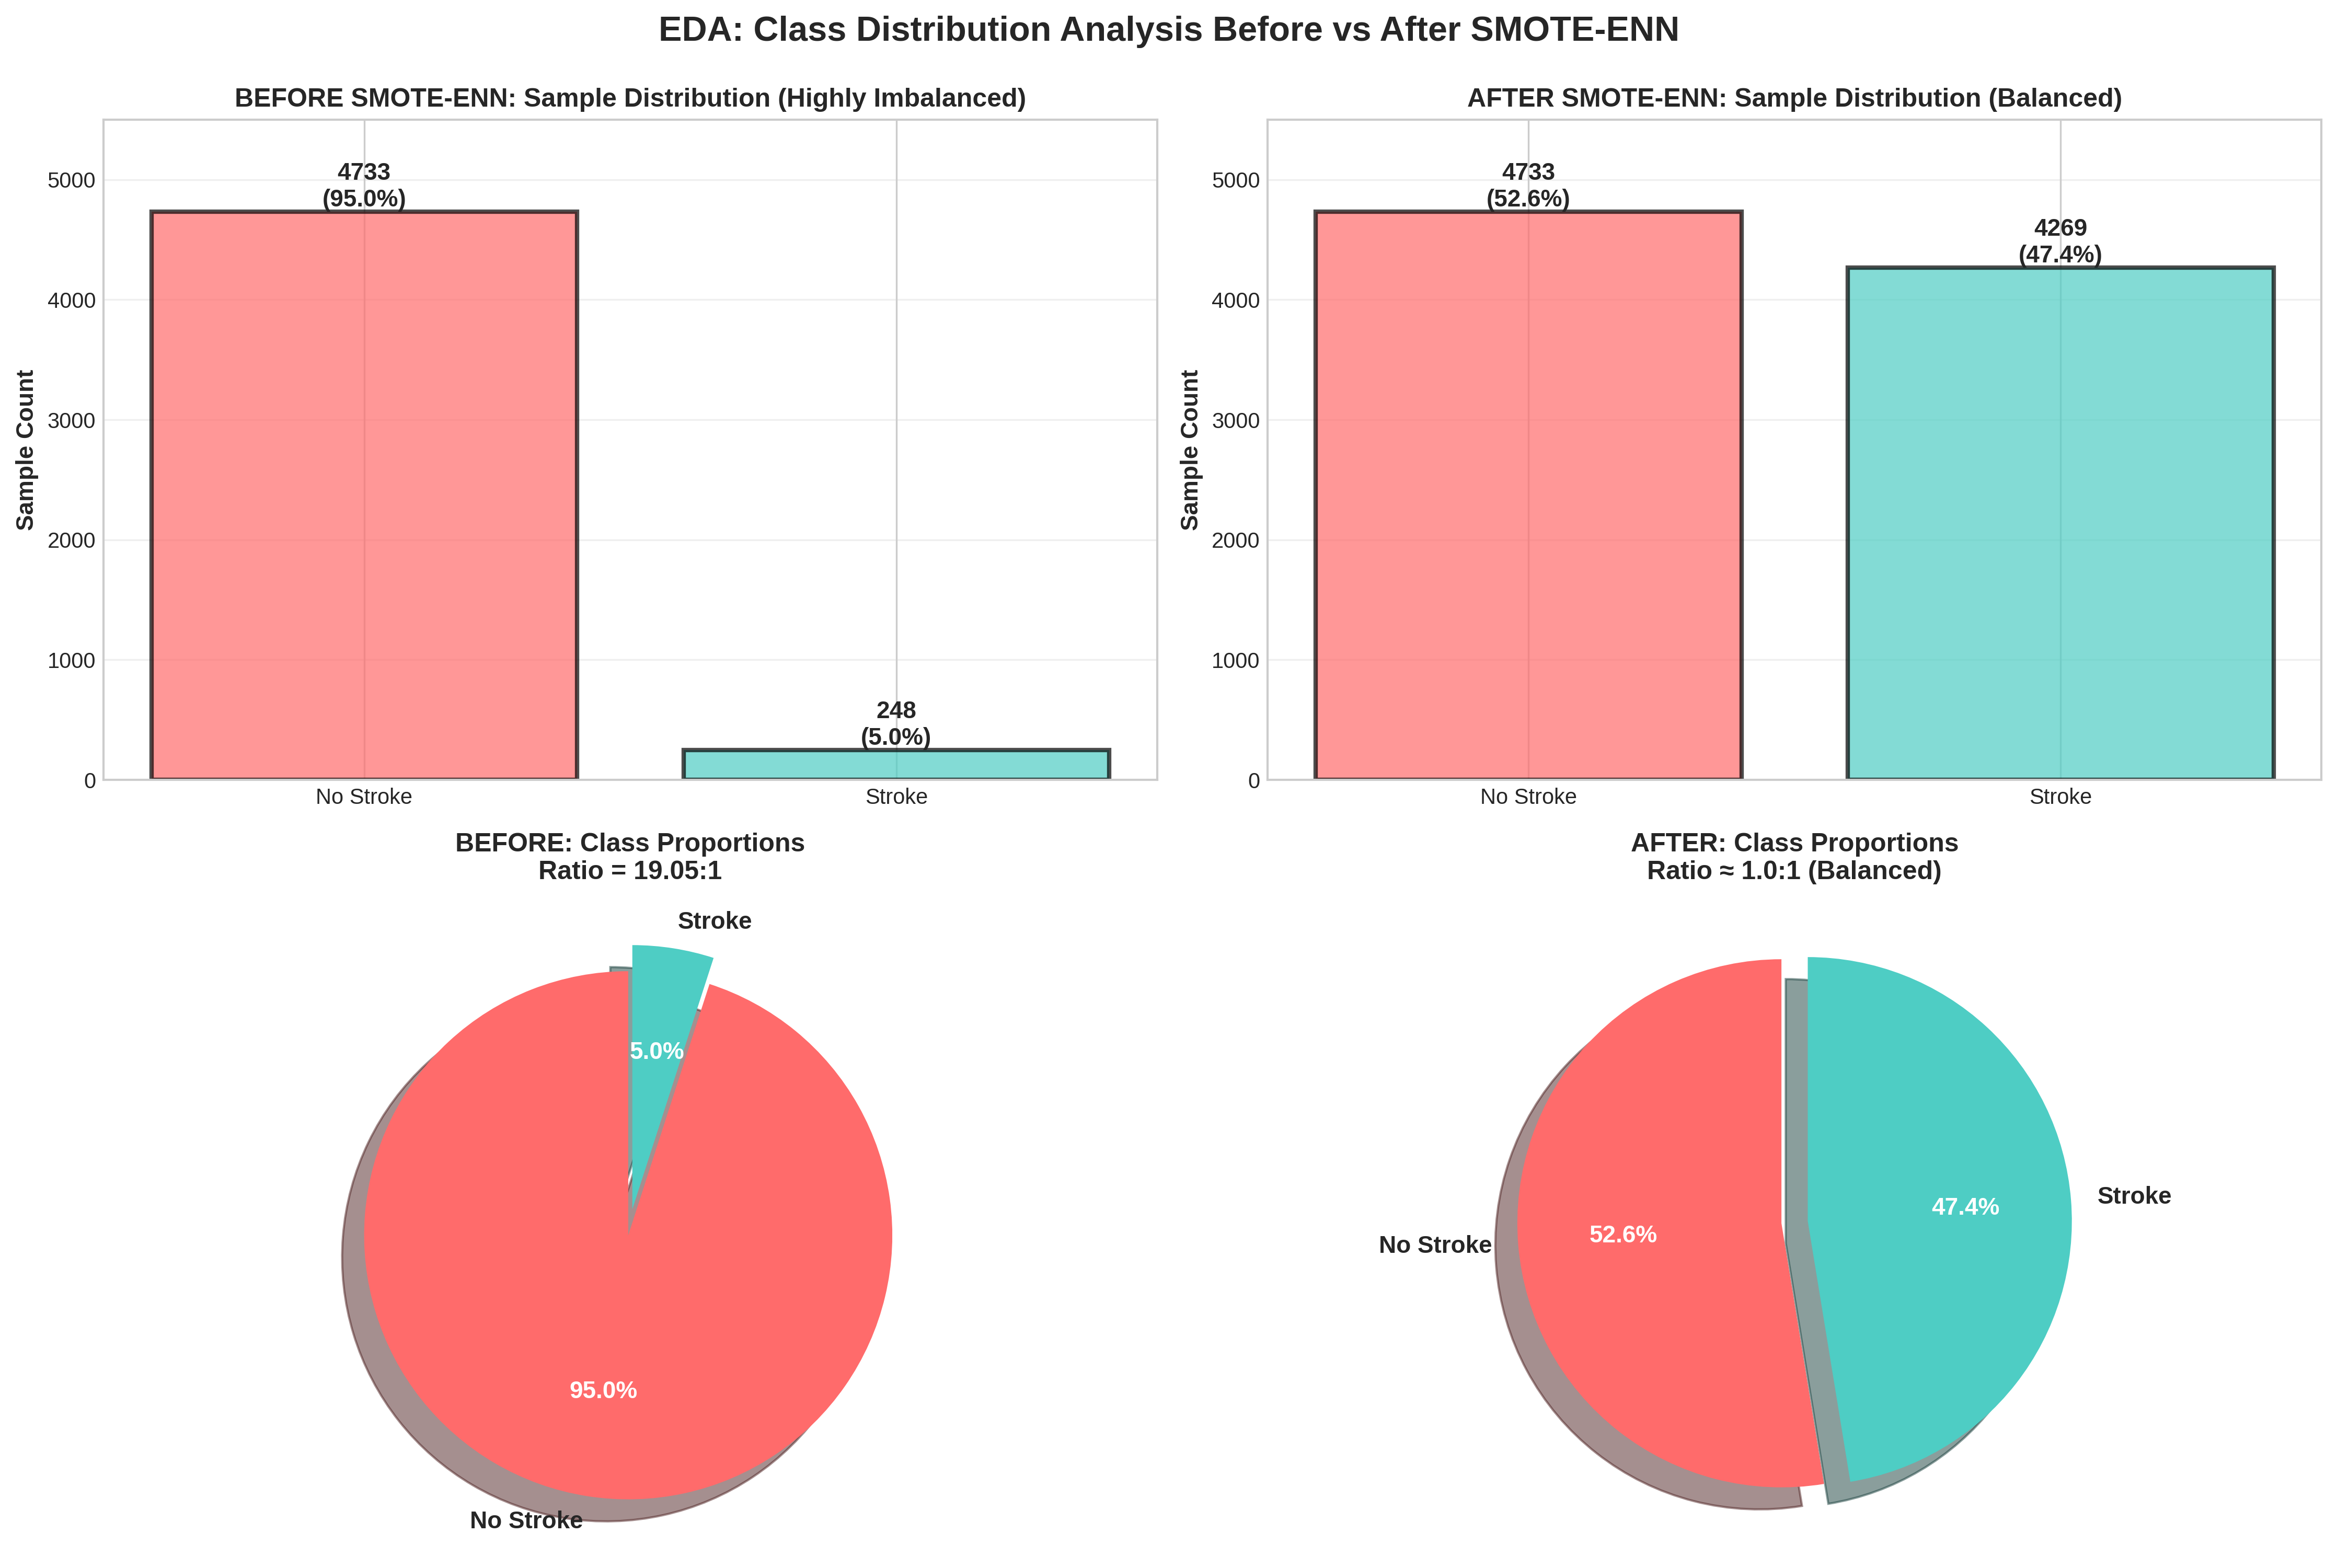
\includegraphics[width=\textwidth]{figures/fig1_class_distribution.png}}
\caption{Class distribution before and after SMOTE-ENN balancing. The original
cohort contains 248 stroke cases against 4,733 controls (19.05:1); balancing
brings the two classes to approximately equal size. In the evaluation protocol
of Sec.~\ref{sec:protocol} this transformation is applied to training
partitions only}
\label{fig:classdist}
\end{figure}

\begin{figure}[htb]
\centerline{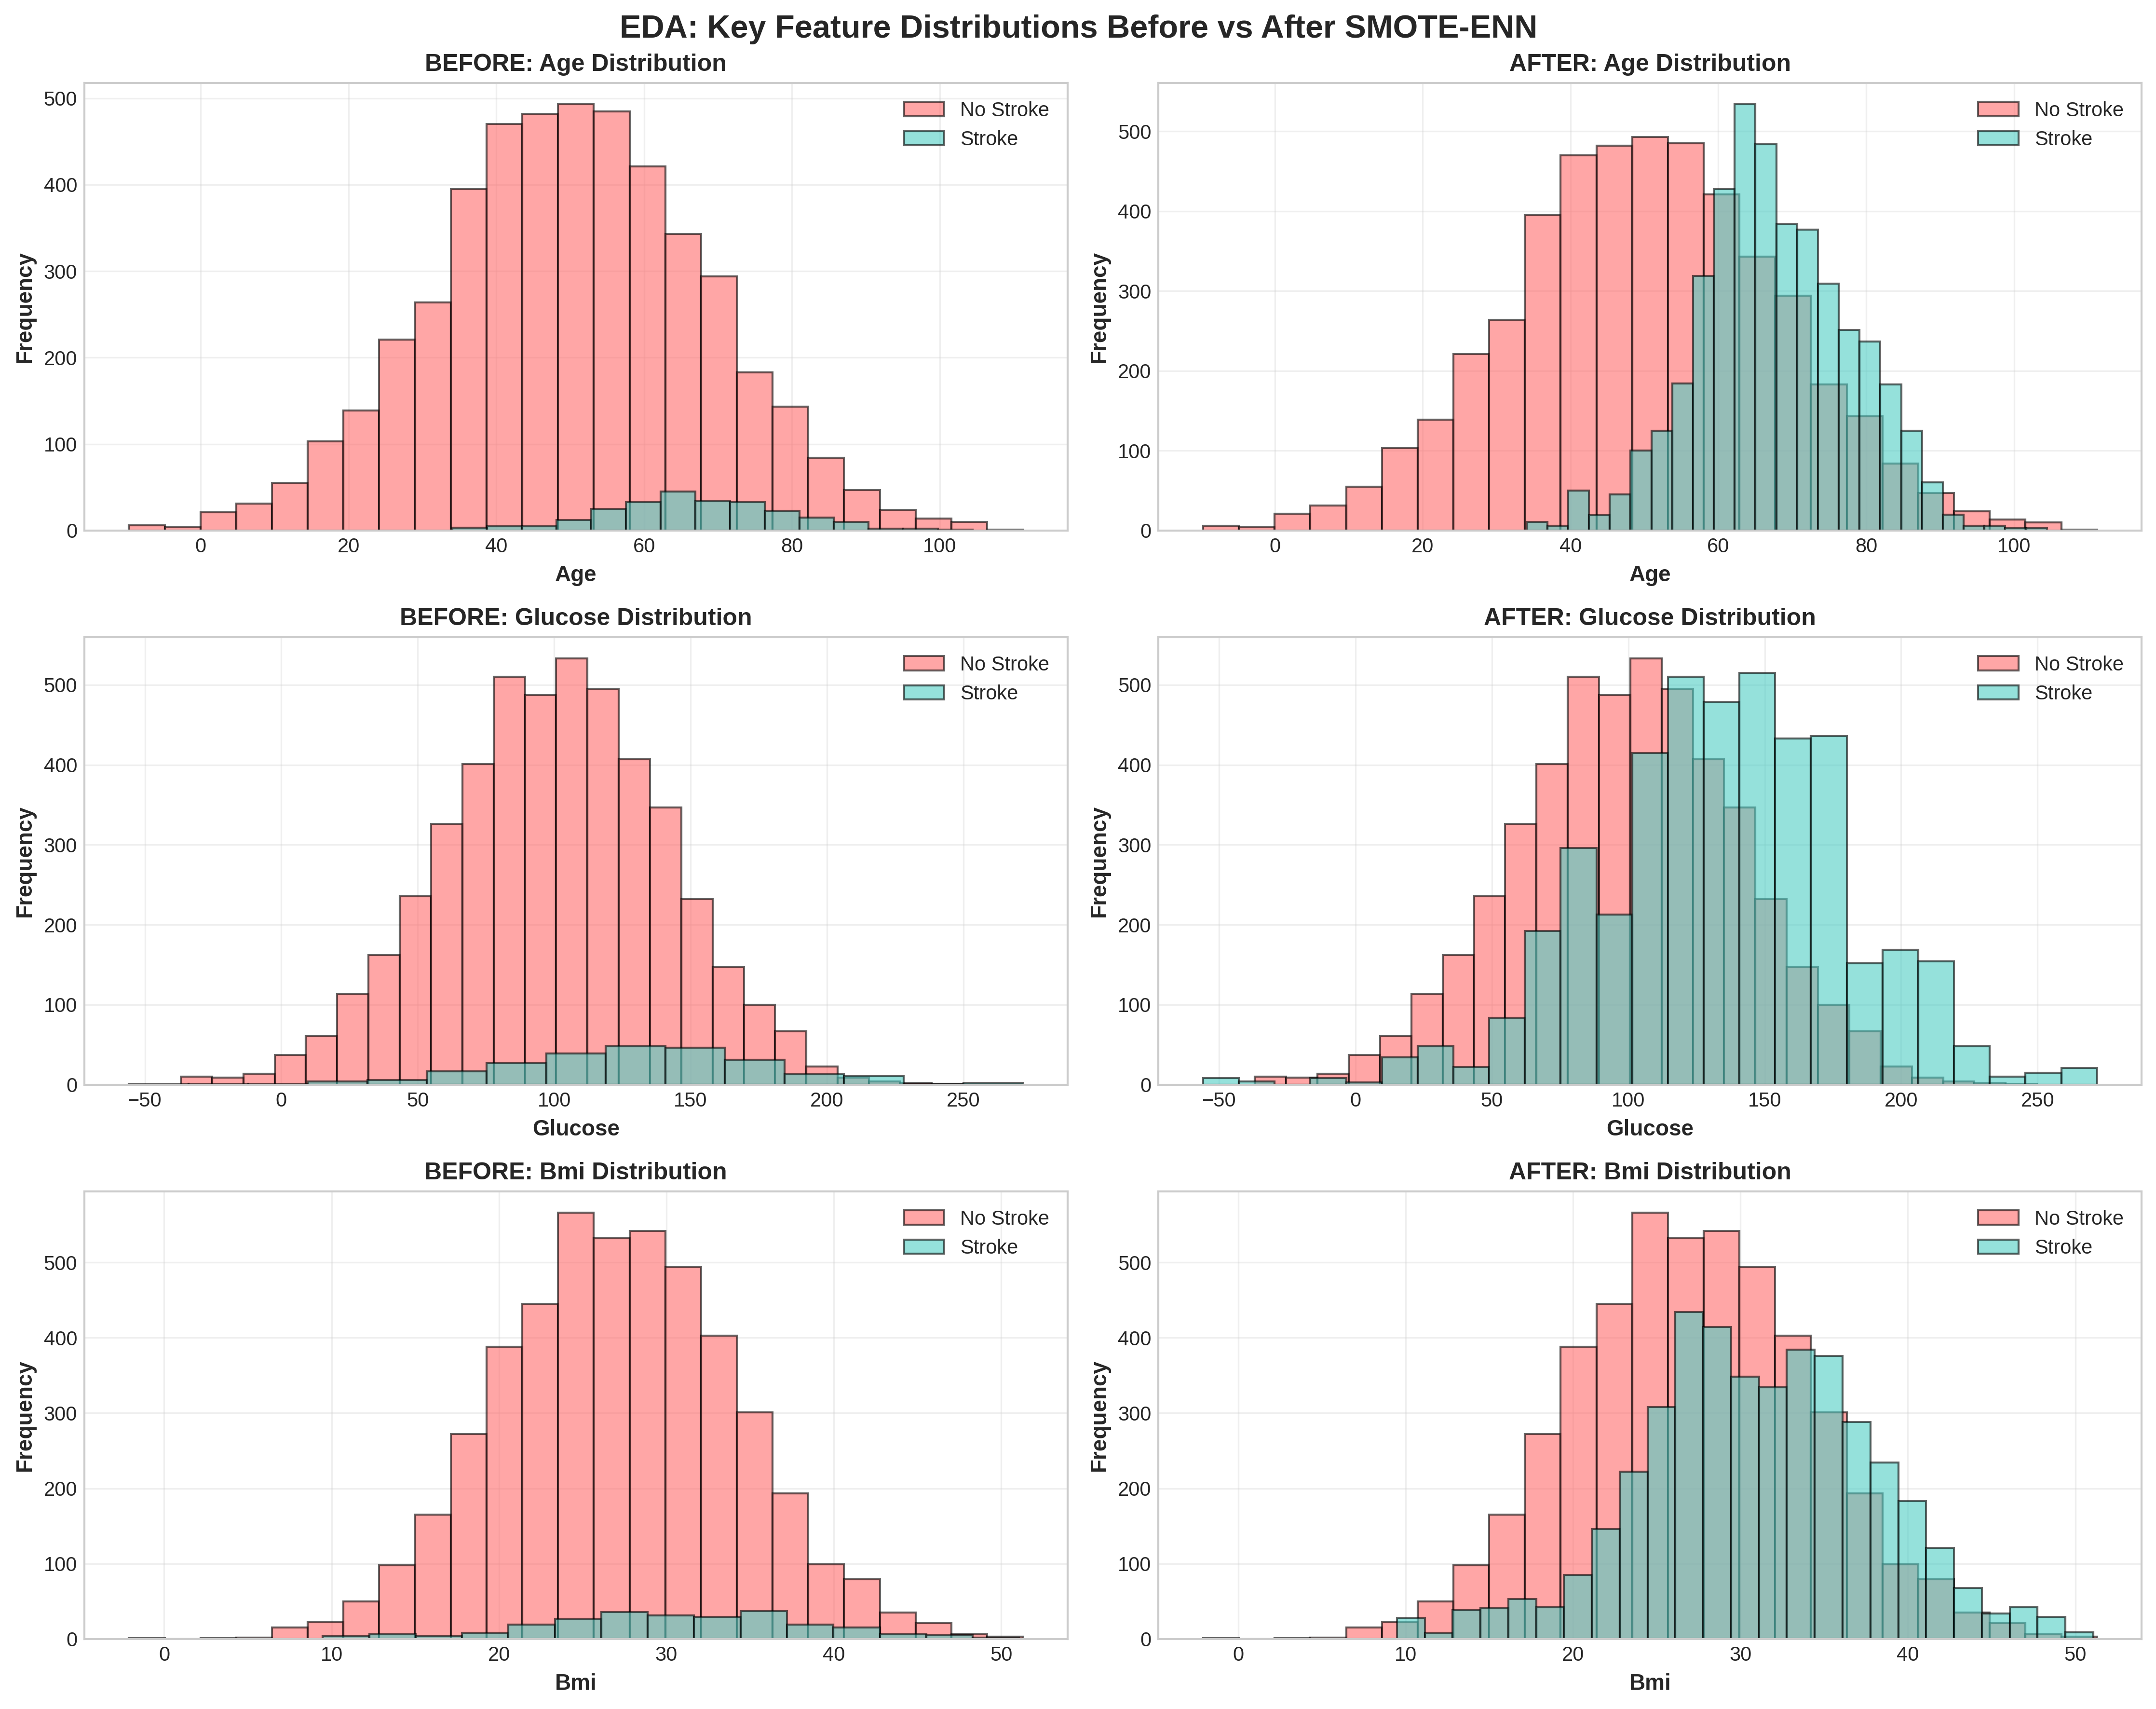
\includegraphics[width=\textwidth]{figures/fig2_feature_distributions.png}}
\caption{Distributions of age, average glucose level and BMI before and after
SMOTE-ENN balancing. Synthetic minority samples remain within clinically
plausible ranges and preserve the between-group separation present in the
original data}
\label{fig:featdist}
\end{figure}

\begin{figure}[htb]
\centerline{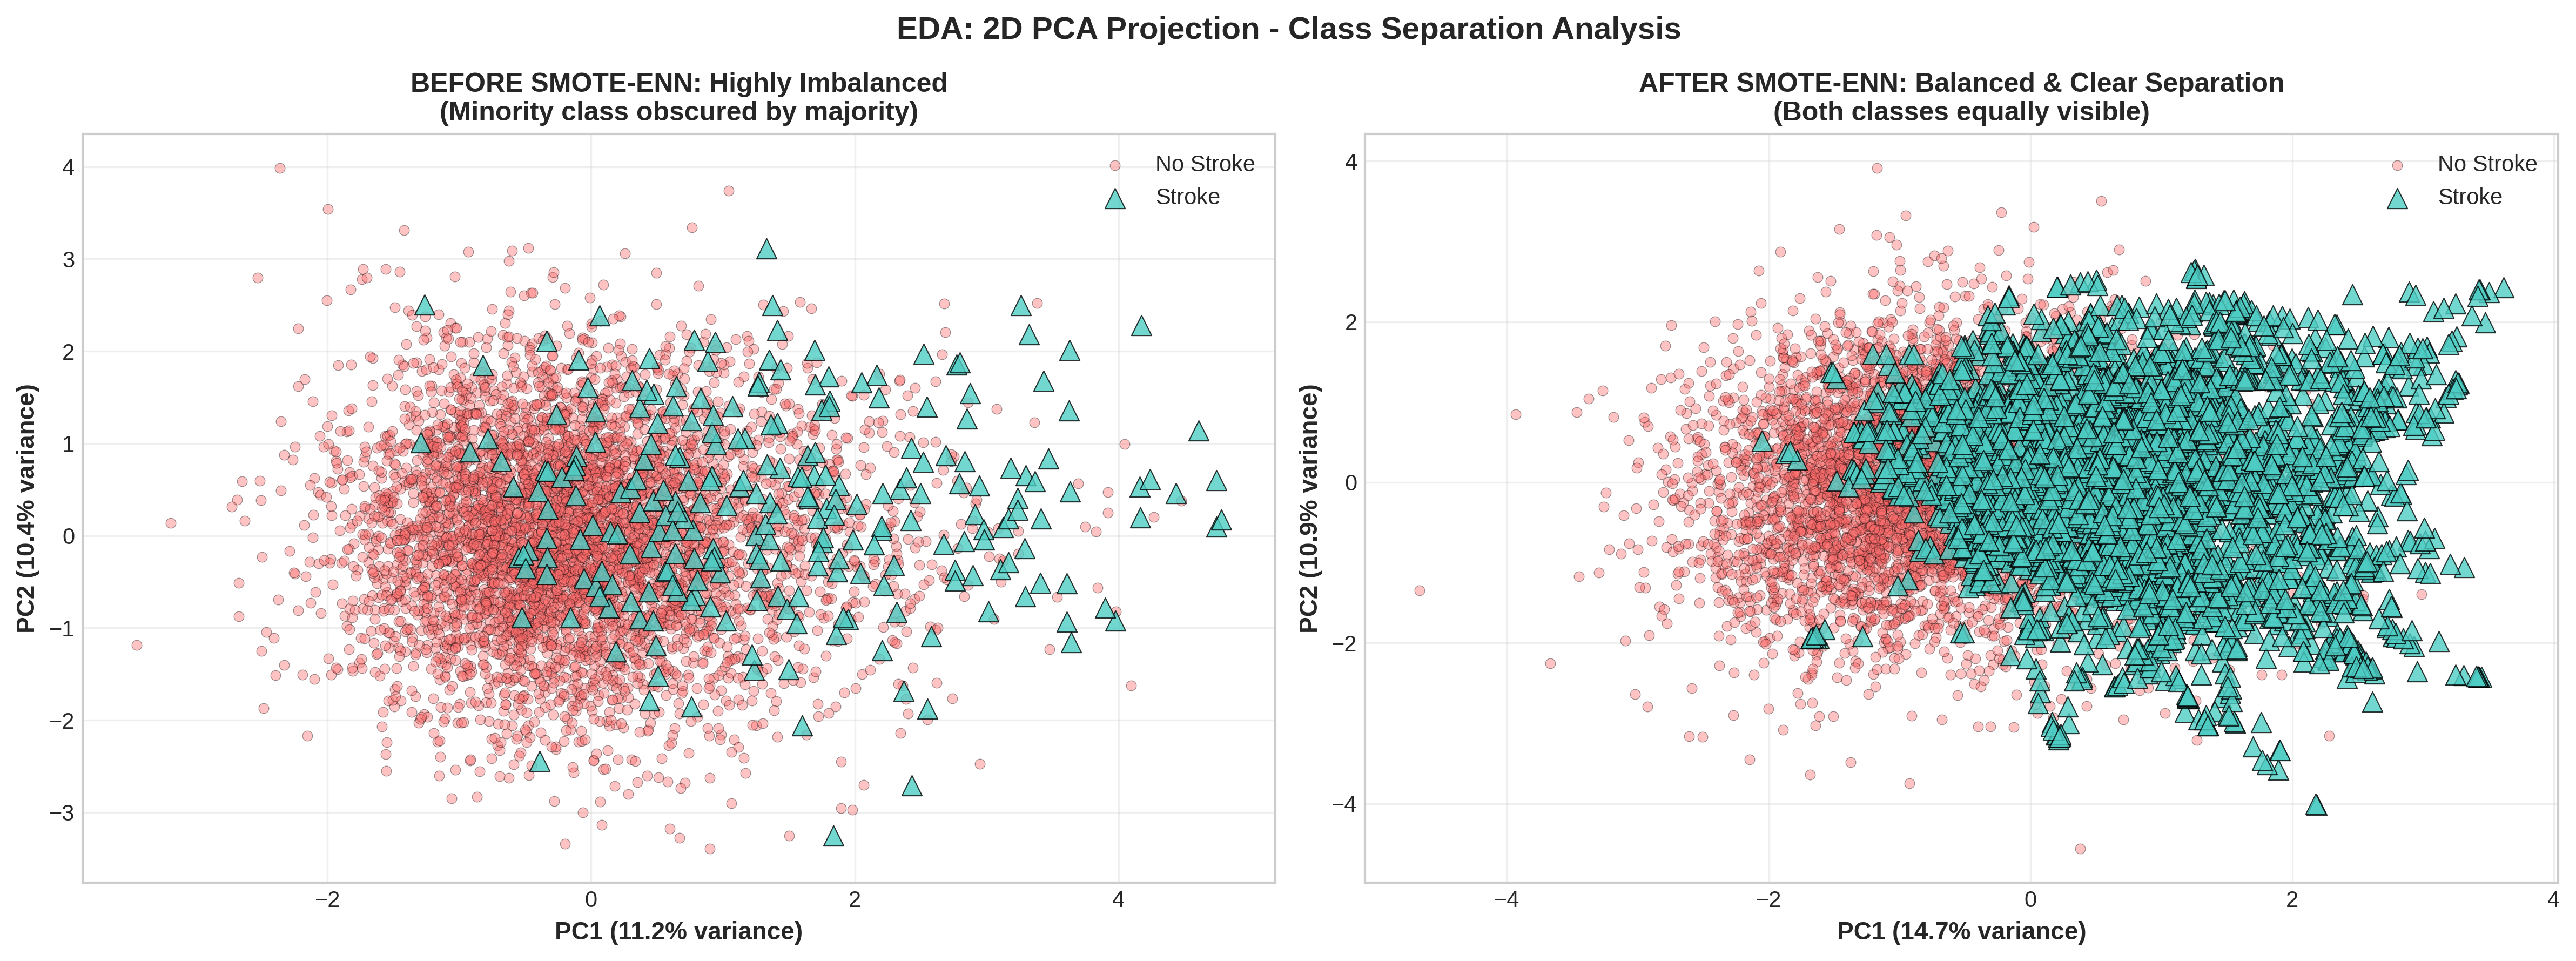
\includegraphics[width=\textwidth]{figures/fig3_pca_projection.png}}
\caption{Two-dimensional PCA projection before and after SMOTE-ENN balancing.
Before balancing the minority class is obscured by the majority class; after
balancing both classes are represented at comparable density}
\label{fig:pca}
\end{figure}

\subsection{Feature Selection}
\label{sec:features}

A five-qubit register admits five angle-encoded features. We select the five
clinically established stroke risk factors---age, average glucose level, BMI,
hypertension status and heart disease history---which are primary drivers of
ischemic stroke in the clinical literature.\cite{howard2012,wolf1991} This is a
clinically motivated choice rather than a purely statistical one, and we report
the corresponding Random Forest importances so that the trade-off is explicit.

On the original imbalanced data, a Random Forest (100 trees, averaged over
three seeds) assigns the importances shown in Fig.~\ref{fig:rfimp}. The five
selected features together account for \textbf{80.1\%} of total importance.
They are not, however, the five features the Random Forest itself ranks
highest: the forest ranks average glucose (0.2845), BMI (0.2425), age (0.2269),
smoking status (0.0689) and work type (0.0472) as its top five, cumulatively
87.0\%. Hypertension (0.0249) and heart disease (0.0225) rank eighth and ninth
despite their established clinical role, a consequence of their low prevalence
and binary coding. We retain the clinical selection, and Table~\ref{tab:qubit}
records the importance of each encoded feature.

\begin{figure}[htb]
\centerline{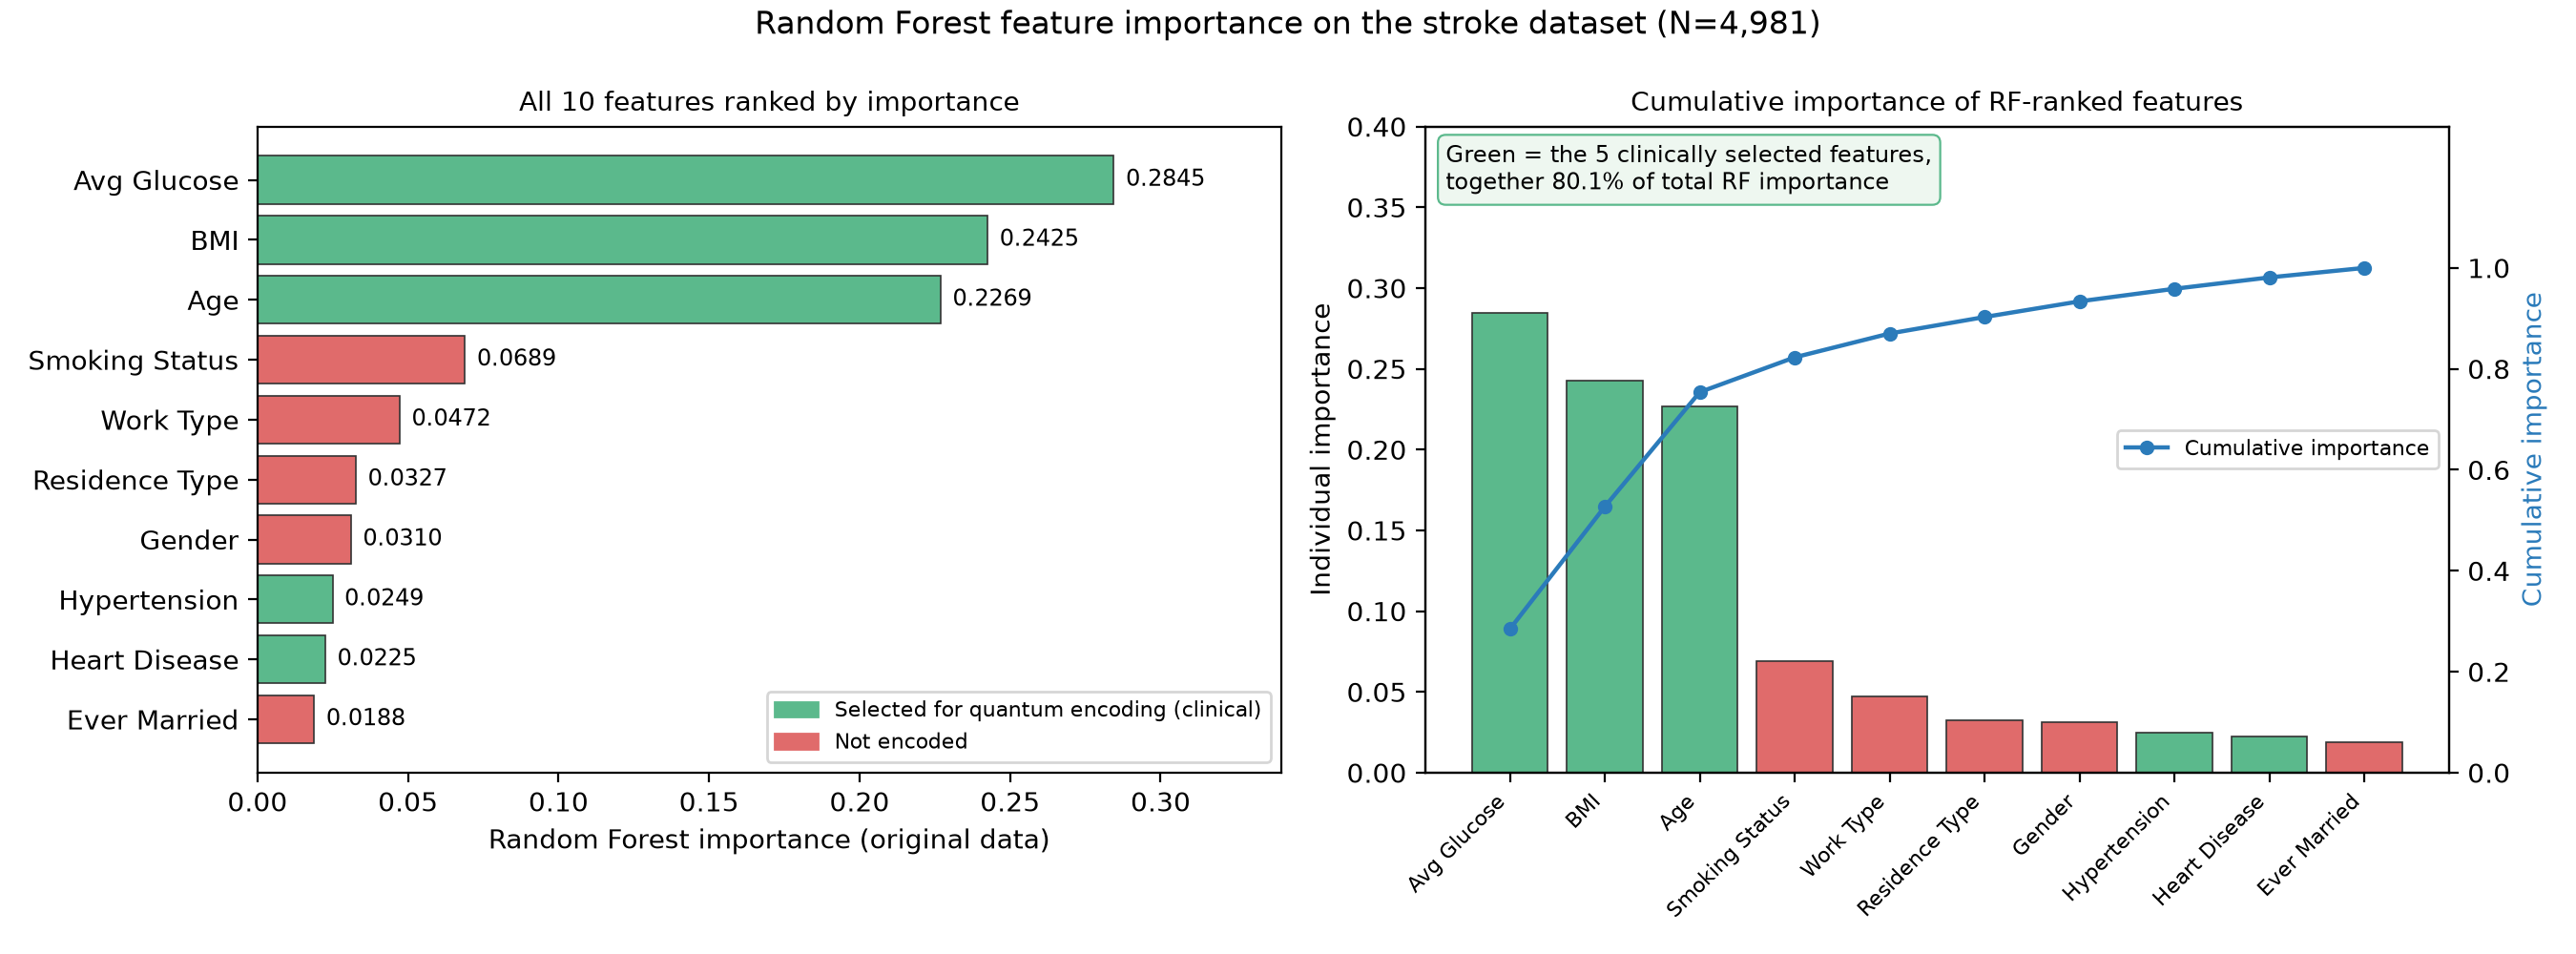
\includegraphics[width=\textwidth]{figures/fig4_rf_importance.png}}
\caption{Random Forest feature importance on the original stroke dataset
($N=4{,}981$), averaged over three seeds. Left: all 10 features ranked by
importance, with the five clinically selected features in green. Right:
individual and cumulative importance of the RF-ranked features. The five
selected features account for 80.1\% of total importance, but are not
identical to the five the forest ranks highest}
\label{fig:rfimp}
\end{figure}

\begin{figure}[htb]
\centerline{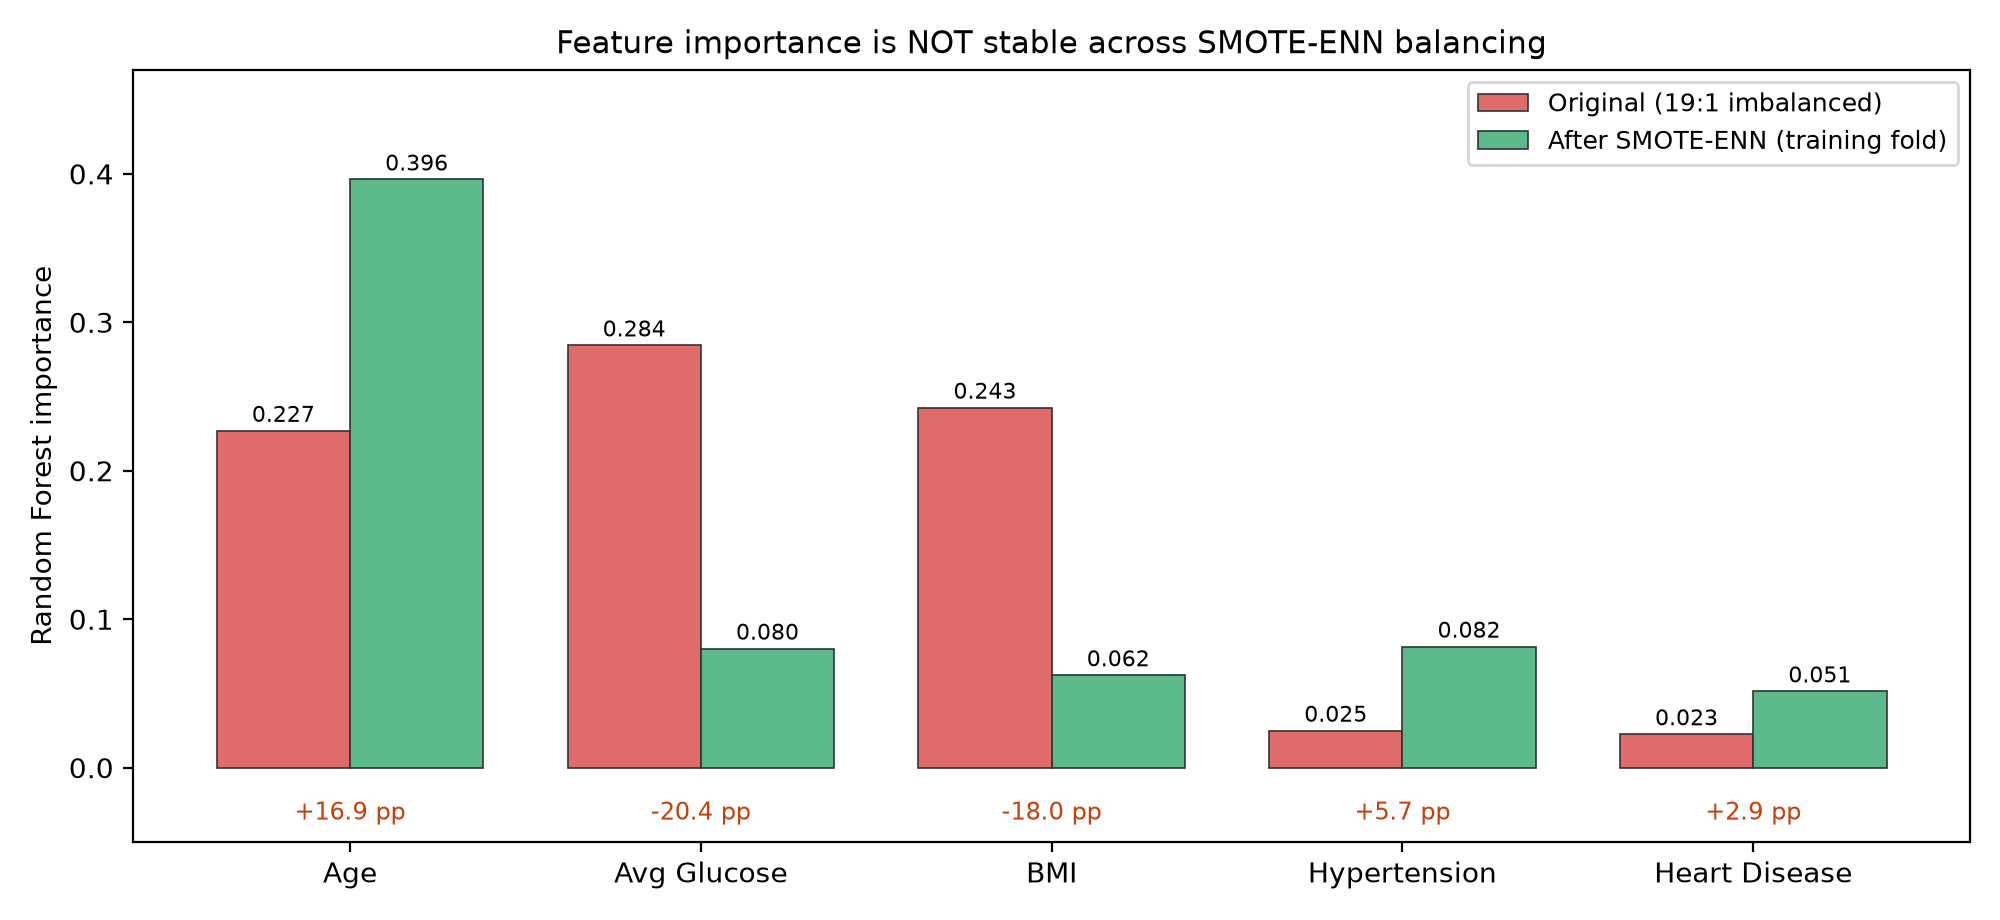
\includegraphics[width=0.92\textwidth]{figures/fig5_importance_shift.png}}
\caption{Random Forest importance of the five encoded features on the original
imbalanced data (red) against SMOTE-ENN balanced data (green), averaged over
three seeds. Importance is \emph{not} stable across balancing: age gains
16.9~pp while average glucose and BMI lose 20.4~pp and 18.0~pp respectively.
Feature importances measured after resampling therefore cannot be used to
justify a feature selection intended to describe the original clinical
population}
\label{fig:impshift}
\end{figure}

A cautionary observation follows from Fig.~\ref{fig:impshift}. Random Forest
importances are markedly \emph{not} invariant under SMOTE-ENN balancing. On the
balanced data the same five features account for only 67.2\% of total
importance, and individual scores shift substantially: age rises from 0.227 to
0.396 ($+16.9$~pp) while average glucose falls from 0.284 to 0.080
($-20.4$~pp) and BMI from 0.243 to 0.062 ($-18.0$~pp), the largest single
shift across all ten features. Synthetic oversampling densifies the
minority class along interpolation directions and thereby changes which splits
reduce impurity, so importance rankings computed after balancing describe the
resampled distribution rather than the clinical population. Feature selection
and its justification should therefore be reported on the original data, as
they are here.

\subsection{Quantum Circuit Design}
\label{sec:circuit}

The five selected features are embedded into a five-qubit register. For a
system of $n$ qubits the state space dimension is
\begin{equation}
\dim(\mathcal{H}) = 2^{n},
\label{eq:dim}
\end{equation}
so that with $n=5$,
\begin{equation}
\dim(\mathcal{H}) = 2^{5} = 32 .
\label{eq:dim32}
\end{equation}
The encoded state is a superposition over all 32 computational basis states,
\begin{equation}
|\psi(x)\rangle = \sum_{s=0}^{31} c_s(x)\,|s\rangle ,
\label{eq:state}
\end{equation}
where the complex amplitudes $c_s(x)$ satisfy
\begin{equation}
\sum_{s=0}^{31} |c_s(x)|^2 = 1 .
\label{eq:norm}
\end{equation}

The circuit comprises \emph{two} layers and a total of 15 gates at depth 3. It
contains no trainable parameters.

\vspace{4pt}
\noindent\textbf{Layer 1: Feature encoding (10 gates, depth 2).}
Each normalised feature $\tilde{x}_i$ is encoded on qubit $i$ by a pair of
rotations,
\begin{equation}
U^{(i)}_{\mathrm{encode}} = R_z(\theta_i)\,R_y(\theta_i),
\label{eq:encode}
\end{equation}
where the $R_y$ gate encodes the feature amplitude and $R_z$ contributes phase
information. Features are min--max scaled to $[-1,1]$ on the training partition,
\begin{equation}
\tilde{x}_i = \frac{2\,(x_i - x_i^{\min})}{x_i^{\max} - x_i^{\min}} - 1 ,
\label{eq:scale}
\end{equation}
with $x_i^{\min}$ and $x_i^{\max}$ taken from the training fold only and test
values clipped to $[-1,1]$, and the rotation angle is
\begin{equation}
\theta_i = \pi\,\tilde{x}_i .
\label{eq:angle}
\end{equation}
Equation~(\ref{eq:angle}) is the single encoding used throughout this work and
matches the released implementation exactly.

\vspace{4pt}
\noindent\textbf{Layer 2: CNOT ring entanglement (5 gates, depth 1).}
A circular CNOT topology
\[
Q_0 \rightarrow Q_1 \rightarrow Q_2 \rightarrow Q_3 \rightarrow Q_4 \rightarrow Q_0
\]
correlates the encoded features, where each gate is
\begin{equation}
\mathrm{CNOT}_{c\to t} = |0\rangle\langle 0|_c \otimes I_t
                       + |1\rangle\langle 1|_c \otimes X_t .
\label{eq:cnot}
\end{equation}
The ring closure ensures that every encoded feature participates in at least
two entangling operations.

\subsubsection{Feature-to-qubit assignment}

Table~\ref{tab:qubit} records the assignment of clinical features to qubits
together with their Random Forest importance on the original data.

\begin{table}[htb]
\tbl{Feature-to-qubit assignment for the five-qubit quantum kernel model.
Importances are Random Forest scores on the original (unbalanced) dataset,
averaged over three seeds.}
{\fontsize{8}{10}\selectfont
\begin{tabular}{@{}llc>{\raggedright\arraybackslash}p{1.75in}@{}}
\toprule
Qubit & Feature & RF imp. & Clinical significance \\
\colrule
$Q_0$ & Age & 0.2269 & Strongest continuous predictor; risk rises
                       steeply beyond 65 \\
$Q_1$ & Avg.\ glucose & 0.2845 & Hyperglycaemia ($\geq$125~mg/dL);
                       metabolic syndrome \\
$Q_2$ & BMI & 0.2425 & Obesity ($\geq$30~kg/m$^2$); modifiable
                       risk factor \\
$Q_3$ & Hypertension & 0.0249 & Diagnosed hypertension (binary) \\
$Q_4$ & Heart disease & 0.0225 & Cardiac comorbidity (binary);
                       cardioembolic pathway \\
\colrule
Total & (5 features) & 0.8013 & 80.1\% of total RF importance \\
\botrule
\end{tabular}}
\label{tab:qubit}
\end{table}

\subsection{Mathematical Formulation}
\label{sec:math}

\subsubsection{The fidelity kernel}

The classical radial basis function (RBF) kernel measures similarity through
Euclidean distance,
\begin{equation}
K_{\mathrm{RBF}}(x_i,x_j) = \exp\!\left(-\gamma\,\|x_i-x_j\|^2\right),
\label{eq:rbf}
\end{equation}
with kernel width $\gamma$. The proposed quantum kernel is the squared overlap
of the two encoded states,
\begin{equation}
K_{Q}(x_i,x_j) = \big|\langle \phi(x_i) | \phi(x_j)\rangle\big|^{2},
\label{eq:qkernel}
\end{equation}
where $|\phi(x)\rangle$ is the state produced by Layers 1 and 2 of
Sec.~\ref{sec:circuit}.

Equation~(\ref{eq:qkernel}) is evaluated by the adjoint (overlap) method: both
statevectors are computed and their inner product taken directly. This requires
a single five-qubit register and no ancilla. We note this explicitly because
the alternative SWAP-test estimator, which is frequently quoted in this
setting, would require $5+5+1=11$ qubits to compare two five-qubit states and
would therefore substantially weaken rather than support a NISQ-feasibility
argument. The resulting $N\times N$ kernel matrix is supplied to a classical
SVM with a pre-computed kernel.

\subsubsection{Kernel concentration}

A quantum kernel is only useful if its values are informative. Thanasilp
\textit{et al.}\cite{thanasilp2024} show that for many feature-map families the
off-diagonal kernel values concentrate exponentially in the number of qubits
towards a fixed value, so that
\begin{equation}
\mathrm{Var}_{i\neq j}\big[K_Q(x_i,x_j)\big] \in \mathcal{O}(b^{-n}),
\qquad b>1 ,
\label{eq:conc}
\end{equation}
which destroys the kernel's ability to discriminate and requires an
exponentially growing number of measurement shots. Because the effect is
exponential in $n$, a circuit of only five qubits is expected to lie well
outside the concentrated regime. We verify this empirically in
Sec.~\ref{sec:qresults} by measuring the off-diagonal spread and numerical rank
of the training kernel matrices.

\subsubsection{Sources of any quantum--classical difference}
\label{sec:advantage}

It is sometimes argued that a quantum feature map benefits from operating in a
higher-dimensional space than a classical kernel. This argument does not hold
for the RBF kernel. The reproducing kernel Hilbert space (RKHS) induced by
$\exp(-\gamma\|x-y\|^2)$ is \emph{infinite}-dimensional, as the Mercer
expansion of the Gaussian makes explicit; the 32-dimensional space of five
qubits is vastly smaller, not larger. Dimensionality therefore cannot be the
source of any advantage here.

What distinguishes the two kernels is their inductive bias. The angle-encoding
map induces a specific, structured inner product on a compact 32-dimensional
space, in which the CNOT ring imposes an explicit entanglement structure: the
$Q_0\!\to\!Q_1$ coupling ties age to glucose, the chain
$Q_1\!\to\!Q_2\!\to\!Q_3$ relates glucose, BMI and hypertension, and the ring
closure $Q_4\!\to\!Q_0$ links cardiac comorbidity back to age. These
multiplicative interactions are captured without manual feature engineering.
Any performance difference between the quantum and classical kernels reported
below must accordingly be attributed to this difference in inductive bias, not
to Hilbert space dimensionality.

Whether such a bias helps is an empirical question, and the prevailing
theoretical picture counsels caution: Huang \textit{et al.}\cite{huang2021}
show that classical learners given access to data can match quantum models
across a wide range of tasks, so that a quantum feature map confers an
advantage only where its bias genuinely matches the target function.

For the same reason we make no claim that amplitude normalisation,
Eq.~(\ref{eq:norm}), provides a quantum-specific regulariser. Every normalised
kernel satisfies $K(x,x)=1$, including the RBF kernel; the constraint is a
property of normalisation, not of quantum mechanics. The relevant statement is
weaker and purely structural: the compact 32-dimensional feature map imposes a
form of implicit dimensionality control.

\subsubsection{NISQ resource requirements}
\label{sec:nisq}

The circuit requires 5 qubits, 15 gates (10 single-qubit rotations and 5 CNOTs)
and depth 3. This is comfortably within the coherence budget of all current
NISQ platforms, and the gate set---parameterised single-qubit rotations and
CNOT---compiles natively on superconducting and trapped-ion hardware.

Encoding all 10 available features would require a 10-qubit register with
\begin{equation}
\dim(\mathcal{H}) = 2^{10} = 1{,}024
\label{eq:dim1024}
\end{equation}
basis states and roughly 30 gates, and would move the circuit materially closer
to the concentration regime of Eq.~(\ref{eq:conc}). The five-feature choice is
thus motivated by both hardware economy and kernel conditioning.

Because the feature map is fixed, kernel entries are computed by forward
circuit evaluation alone. No variational parameters are trained, no
gradients are estimated, and the barren plateau phenomenon\cite{mcclean2018}
does not arise: it is a property of parameter landscapes, and this model has
none.

\subsection{Evaluation Protocol and Leakage Prevention}
\label{sec:protocol}

The order of resampling and splitting determines whether a cross-validation
estimate is meaningful. Under the \emph{leaky} protocol---the one used in most
prior work on this dataset, including our own\cite{shinde2024}---SMOTE-ENN is
applied to the entire dataset and the balanced result is then partitioned into
folds. Because SMOTE synthesises minority points by interpolating between
existing minority samples, a synthetic point derived in part from a test
patient can be placed in the training set. The test fold is then no longer
independent of training, and minority-class recall in particular is inflated.
ENN compounds the problem by deleting exactly those minority points that are
hardest to classify, including from what will become the test fold.

Under the \emph{leakage-free} protocol used for our primary results, the
original imbalanced data are partitioned first, using stratified five-fold
cross-validation, and SMOTE-ENN is then applied inside each training fold only.
The min--max scaler is likewise fitted on the training fold alone. Each held-out
fold therefore contains 996--997 original patients at natural prevalence
(946--947 controls, 49--50 stroke cases). Cross-validation is repeated over
three random seeds, giving 15 folds in total; all results are reported as
mean~$\pm$ standard deviation over those 15 folds.

We evaluate both protocols on identical models and identical data so that the
inflation attributable to resampling order can be quantified directly
(Sec.~\ref{sec:ablation}). Reporting both is the second contribution of this
work.

%%%%%%%%%%%%%%%%%%%%%%%%%%%%%%%%%%%%%%%%%%%%%%%%%%%%%%%%%%%%%%%%%%%%%%%%%%%%%%
\section{Results}
\label{sec:results}

\subsection{Dataset and Preprocessing Outcomes}
\label{sec:preproc}

The cohort comprises $N=4{,}981$ patients: 248 stroke cases (4.98\%) and 4,733
controls (95.02\%), a ratio of 19.1:1. Applying SMOTE-ENN inside each training
fold produces resampled training sets of 6,098--6,393 samples at approximately
1:1 class ratio across the 15 folds. Held-out folds are never resampled and
retain the original 4.98\% prevalence.

All models are trained and evaluated on identical folds. Because the test
distribution is dominated by controls, raw accuracy is a weak summary here: a
classifier that predicts ``no stroke'' for every patient attains 95.02\%
accuracy. We therefore report AUC, area under the precision--recall curve
(AUPRC), recall and balanced accuracy as the clinically meaningful measures,
and include accuracy for completeness only.

\subsection{Classical Baseline Performance}
\label{sec:classical}

Table~\ref{tab:honest} reports all five classifiers under the leakage-free
protocol. Among classical baselines the RBF-SVM ranks highest by AUC
($0.826\pm0.024$) and by recall ($0.754\pm0.077$), followed by random forest
($0.804\pm0.025$). Random forest attains the highest raw accuracy
($0.852\pm0.010$) but the lowest recall ($0.443\pm0.077$): it achieves that
accuracy largely by predicting the majority class, which is precisely the
behaviour raw accuracy fails to penalise at this prevalence. $k$-nearest
neighbours ($k=5$) and a depth-10 decision tree reach AUC $0.751\pm0.033$ and
$0.717\pm0.031$ respectively.

Precision is low for every model (0.126--0.155). At 4.98\% prevalence and
recall near 0.75, the great majority of positive alerts are necessarily false
positives; this is a property of the base rate, not a defect of any particular
classifier.

\begin{table}[htb]
\tbl{Performance of all five classifiers under the leakage-free protocol
(stratified 5-fold cross-validation $\times$ 3 seeds = 15 folds; SMOTE-ENN
applied inside training folds only). Values are mean $\pm$ standard deviation
over the 15 folds. Rows are ordered by AUC.}
{\fontsize{8}{10}\selectfont\setlength{\tabcolsep}{3.5pt}
\begin{tabular}{@{}lcccccc@{}}
\toprule
Model & AUC & AUPRC & Recall & Precision & Bal.\ acc. & Accuracy \\
\colrule
RBF-SVM       & $\mathbf{0.826\pm0.024}$ & $0.183\pm0.027$ & $0.754\pm0.077$ & $0.138\pm0.014$ & $0.753\pm0.034$ & $0.751\pm0.030$ \\
Random forest & $0.804\pm0.025$ & $0.148\pm0.019$ & $0.443\pm0.077$ & $0.155\pm0.020$ & $0.658\pm0.036$ & $0.852\pm0.010$ \\
KNN ($k=5$)   & $0.751\pm0.033$ & $0.121\pm0.016$ & $0.621\pm0.074$ & $0.134\pm0.012$ & $0.705\pm0.034$ & $0.781\pm0.014$ \\
QSVM          & $0.749\pm0.033$ & $0.151\pm0.030$ & $0.613\pm0.062$ & $0.126\pm0.016$ & $0.693\pm0.029$ & $0.765\pm0.031$ \\
Decision tree & $0.717\pm0.031$ & $0.114\pm0.017$ & $0.562\pm0.071$ & $0.135\pm0.017$ & $0.686\pm0.033$ & $0.797\pm0.024$ \\
\botrule
\end{tabular}}
\label{tab:honest}
\end{table}

\subsection{Quantum Kernel SVM Performance}
\label{sec:qresults}

The five-qubit fidelity kernel attains AUC $0.749\pm0.033$, AUPRC
$0.151\pm0.030$, recall $0.613\pm0.062$ and balanced accuracy
$0.693\pm0.029$. It is statistically indistinguishable from KNN by AUC
($0.751\pm0.033$) and below the RBF-SVM by $0.078$ AUC. Its AUPRC
($0.151\pm0.030$) exceeds that of KNN ($0.121\pm0.016$) and of the decision
tree ($0.114\pm0.017$), and matches random forest ($0.148\pm0.019$), which is
the more relevant comparison at this prevalence.

\vspace{4pt}
\noindent\textbf{Kernel concentration.}
Across the 15 training kernel matrices the off-diagonal entries have mean
$0.248$ and standard deviation $0.238$, and a representative $1200\times1200$
block has numerical rank 1,176--1,179 out of 1,200 at tolerance $10^{-8}$. The
kernel is thus close to full rank and its values are widely spread over
$[0,1]$, showing no sign of the exponential concentration described by
Eq.~(\ref{eq:conc}). This is the expected outcome at $n=5$: concentration in
the sense of \refcite{thanasilp2024} sets in exponentially with qubit count,
and five qubits is far from that limit. The measurement is worth recording
because it establishes that the modest performance reported above is a genuine
property of this feature map's inductive bias, and not an artefact of a
degenerate kernel. It also indicates that the circuit width can be increased
somewhat before concentration becomes the binding constraint.

\subsection{Comparison and Significance}
\label{sec:comparison}

Ordering the five classifiers by AUC under the leakage-free protocol gives
RBF-SVM ($0.826$) $>$ random forest ($0.804$) $>$ KNN ($0.751$) $\approx$ QSVM
($0.749$) $>$ decision tree ($0.717$). Figure~\ref{fig:metrics} shows all seven
metrics for all five models.

\begin{figure}[htb]
\centerline{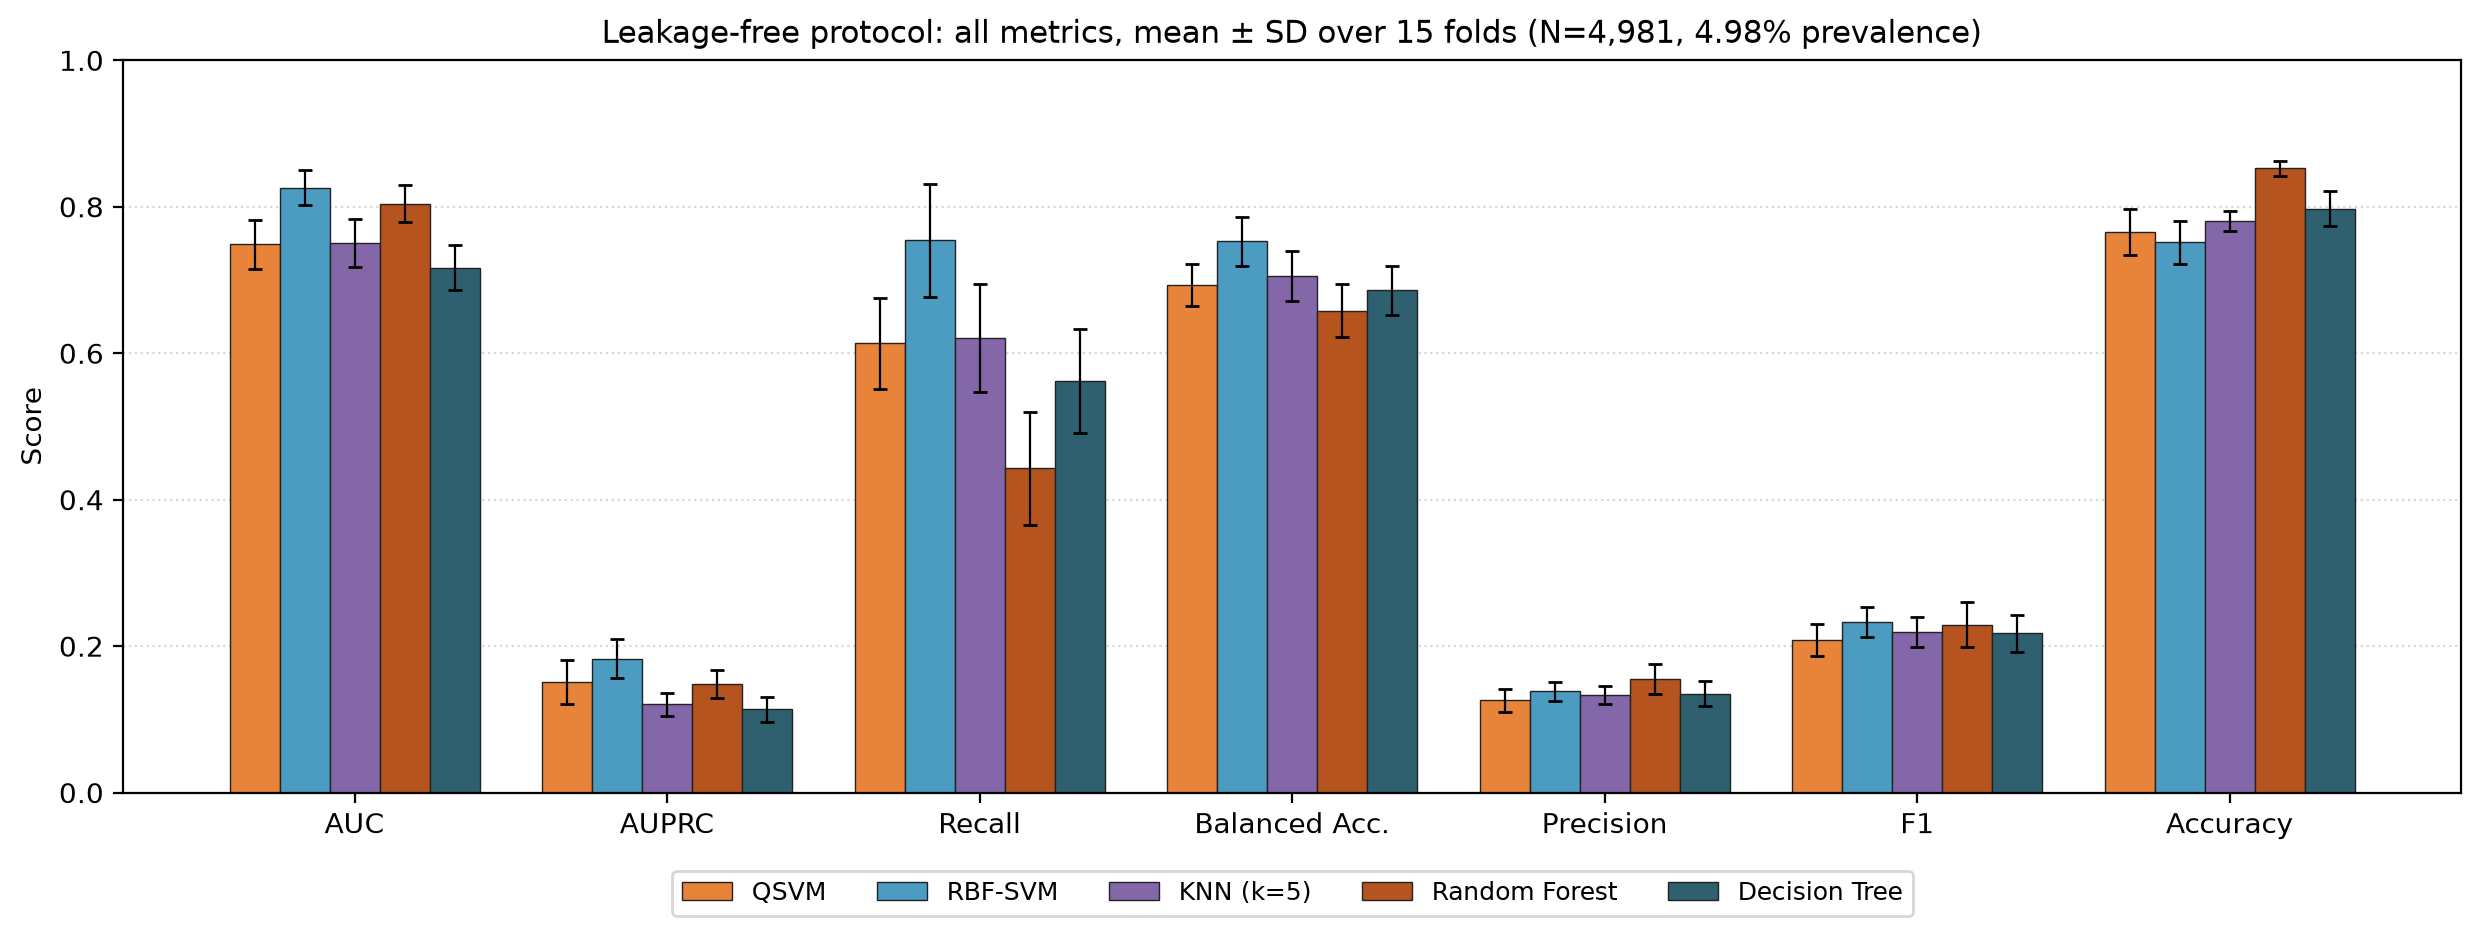
\includegraphics[width=\textwidth]{figures/fig6_metrics_honest.png}}
\caption{All metrics for all five classifiers under the leakage-free protocol,
mean $\pm$ standard deviation over 15 folds. Accuracy is high and nearly
uniform across models because 95.02\% of patients are controls; AUC, AUPRC and
balanced accuracy separate the models meaningfully}
\label{fig:metrics}
\end{figure}

Aggregate metrics do not reveal whether the quantum kernel makes
\emph{different} predictions or merely worse ones. We therefore applied an
exact McNemar test to the paired predictions of the QSVM and the RBF-SVM. For a
single seed the five held-out folds partition the cohort exactly, so each
patient is counted once ($n=4{,}981$). Table~\ref{tab:mcnemar} reports the
discordant pairs for each of the three seeds.

\begin{table}[htb]
\tbl{Exact McNemar test, QSVM against RBF-SVM, under the leakage-free protocol.
For each seed the five held-out folds partition the cohort, so $n=4{,}981$
independent patients. $b$ counts patients the RBF-SVM classifies correctly and
the QSVM does not; $c$ counts the reverse.}
{\fontsize{8}{10}\selectfont
\begin{tabular}{@{}ccccc@{}}
\toprule
Seed & $b$ (classical only) & $c$ (quantum only) & Discordant & Two-sided $p$ \\
\colrule
0 & 288 & 358 & 646 & $6.6\times10^{-3}$ \\
1 & 280 & 339 & 619 & $2.0\times10^{-2}$ \\
2 & 269 & 350 & 619 & $1.3\times10^{-3}$ \\
\botrule
\end{tabular}}
\label{tab:mcnemar}
\end{table}

The direction is consistent across all three seeds and significant at the 5\%
level in each: at the default decision threshold the quantum kernel corrects
more of the RBF-SVM's errors than it introduces. This coexists with a lower
AUC, and the two facts are not in conflict. AUC measures the quality of the
induced ranking over all thresholds, whereas McNemar compares hard decisions at
one threshold. The quantum kernel is therefore better calibrated at the default
threshold but produces a less discriminating ranking function overall. This
nuance---a different decision bias rather than a uniform improvement or
degradation---is the substantive empirical finding of the comparison, and it
would be invisible in either statistic alone.

\subsection{Ablation: Effect of the Resampling Protocol}
\label{sec:ablation}

Table~\ref{tab:ablation} and Fig.~\ref{fig:ablation} compare the two protocols
on identical models and data.

\begin{table}[htb]
\tbl{Effect of resampling protocol. ``Leakage-free'' splits first and applies
SMOTE-ENN inside the training fold; ``leaky'' applies SMOTE-ENN to the full
dataset before splitting. Identical models, folds and seeds; mean $\pm$
standard deviation over 15 folds.}
{\fontsize{8}{10}\selectfont
\begin{tabular}{@{}llcccc@{}}
\toprule
Protocol & Model & AUC & AUPRC & Recall & Bal.\ acc. \\
\colrule
Leakage-free & RBF-SVM       & $0.826\pm0.024$ & $0.183\pm0.027$ & $0.754\pm0.077$ & $0.753\pm0.034$ \\
Leakage-free & Random forest & $0.804\pm0.025$ & $0.148\pm0.019$ & $0.443\pm0.077$ & $0.658\pm0.036$ \\
Leakage-free & QSVM          & $0.749\pm0.033$ & $0.151\pm0.030$ & $0.613\pm0.062$ & $0.693\pm0.029$ \\
\colrule
Leaky        & RBF-SVM       & $0.954\pm0.006$ & $0.961\pm0.005$ & $0.883\pm0.015$ & $0.873\pm0.010$ \\
Leaky        & Random forest & $0.997\pm0.000$ & $0.997\pm0.000$ & $0.980\pm0.007$ & $0.972\pm0.004$ \\
Leaky        & QSVM          & $0.925\pm0.010$ & $0.941\pm0.007$ & $0.841\pm0.023$ & $0.853\pm0.014$ \\
\botrule
\end{tabular}}
\label{tab:ablation}
\end{table}

\begin{figure}[htb]
\centerline{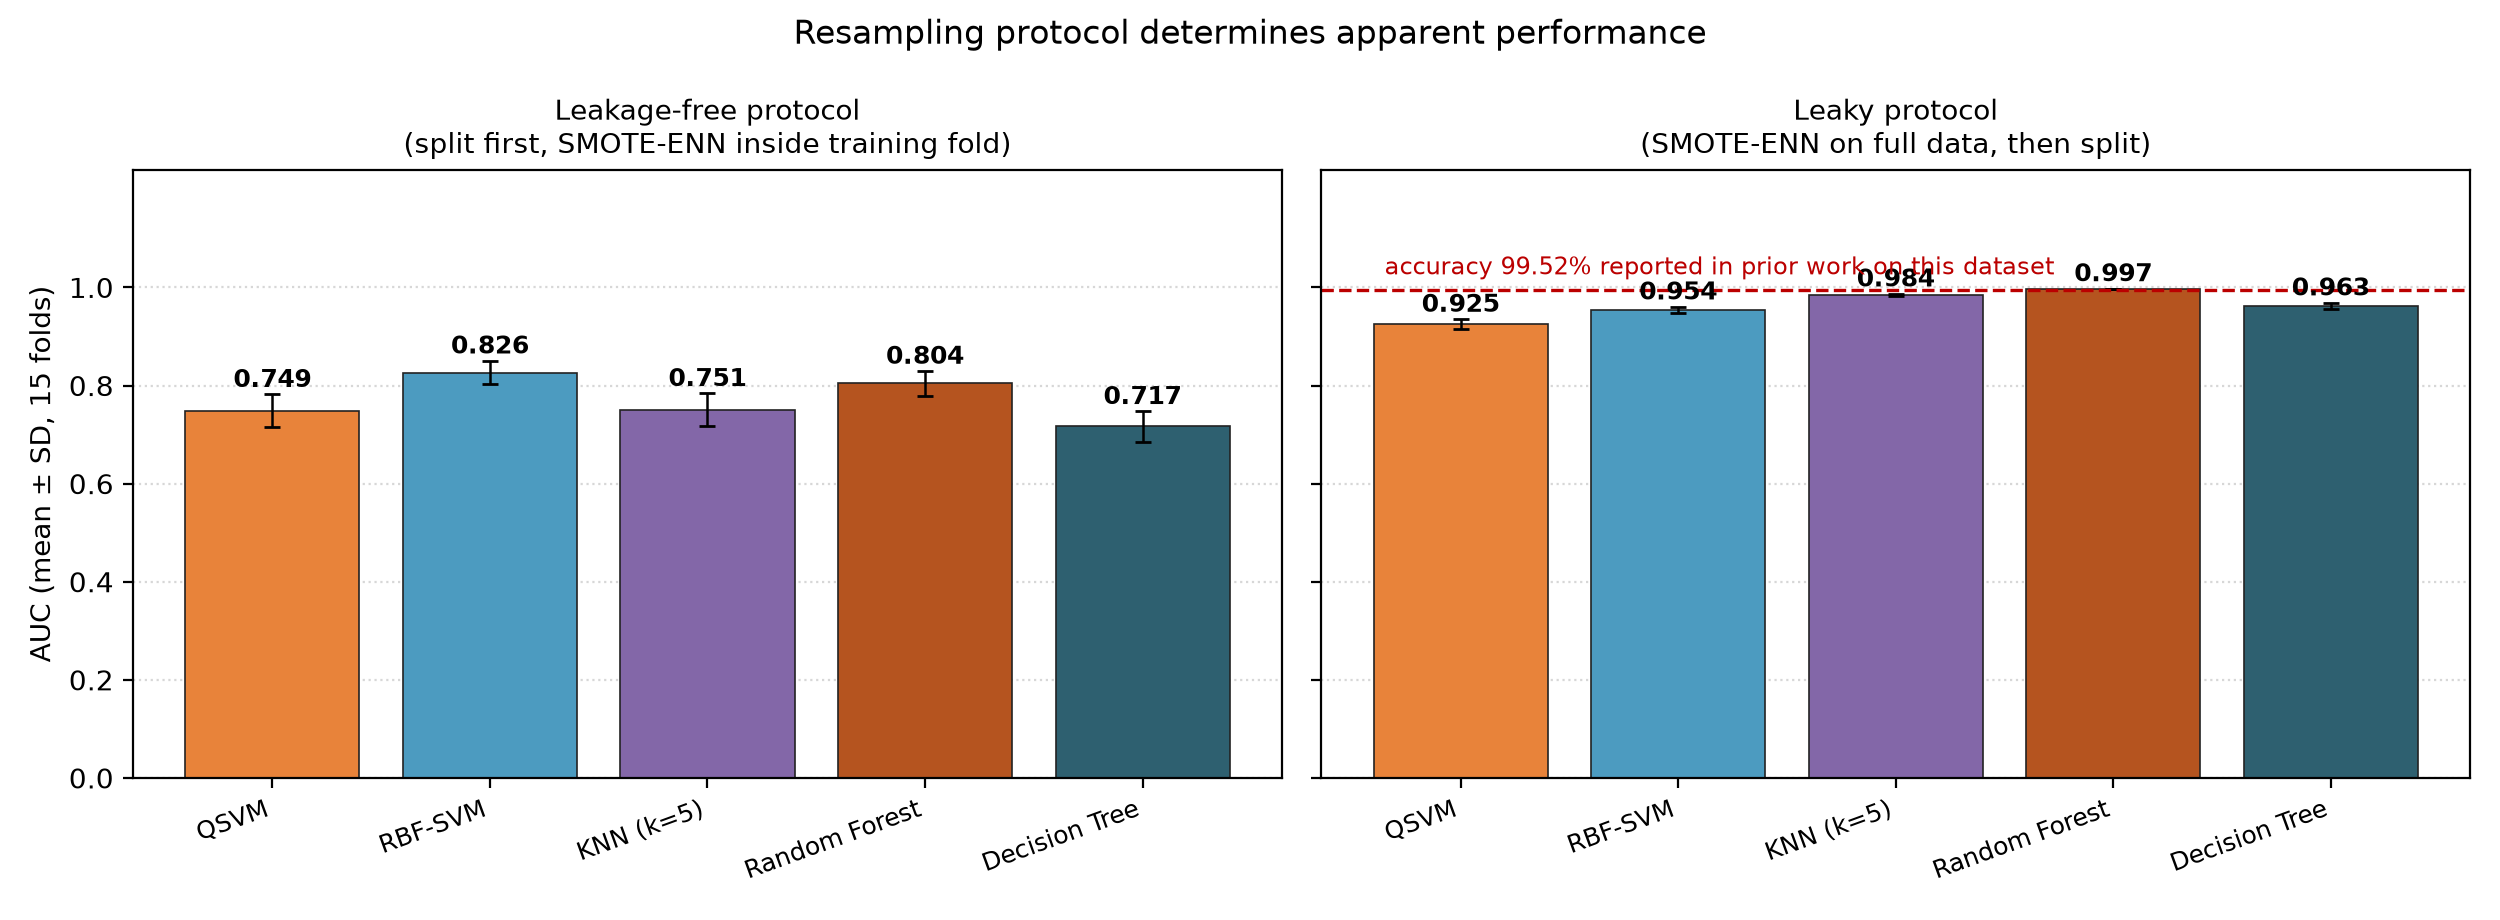
\includegraphics[width=\textwidth]{figures/fig7_protocol_ablation.png}}
\caption{AUC under the two protocols, mean $\pm$ standard deviation over 15
folds. Resampling before splitting raises AUC by 0.13--0.25 for every model and
compresses the between-model differences. The random forest result under the
leaky protocol ($0.997\pm0.000$) is consistent with the 99.52\% accuracy
reported for this dataset in \refcite{shinde2024}}
\label{fig:ablation}
\end{figure}

Applying SMOTE-ENN before splitting inflates AUC by 0.128 (RBF-SVM), 0.177
(QSVM) and 0.193 (random forest), and inflates AUPRC far more dramatically---
from 0.183 to 0.961 for the RBF-SVM, and from 0.151 to 0.941 for the QSVM.
AUPRC is the more sensitive diagnostic because it depends directly on the
positive base rate, which the leaky protocol has silently changed from 4.98\%
to roughly 50\%. Fold-to-fold variability also collapses under the leaky
protocol (for example RBF-SVM AUC standard deviation falls from 0.024 to
0.006), which can easily be mistaken for improved stability.

The random forest reaches AUC $0.997\pm0.000$ and accuracy $0.973\pm0.004$
under the leaky protocol. This is consistent with the 99.52\% accuracy reported
for an eight-model stacking ensemble on this dataset in
\refcite{shinde2024}, whose protocol matches the leaky protocol evaluated
here. We conclude that the previously reported figure reflects resampling
leakage rather than generalisable clinical predictive capability. The same
conclusion applies to the quantum results: a quantum kernel evaluated under the
leaky protocol reaches AUC 0.925, which would be easy to present as a strong
result and is not one.

Two points deserve emphasis. First, the inflation affects classical and quantum
models alike, so a quantum-against-classical comparison conducted entirely
within the leaky protocol is not necessarily wrong in its \emph{ordering}---but
every absolute number it reports is meaningless as an estimate of clinical
performance. Second, the effect is large enough to reverse conclusions: under
the leaky protocol the QSVM appears to be an excellent classifier
(AUC 0.925, recall 0.841); under the leakage-free protocol it is a mediocre one
(AUC 0.749, recall 0.613).

%%%%%%%%%%%%%%%%%%%%%%%%%%%%%%%%%%%%%%%%%%%%%%%%%%%%%%%%%%%%%%%%%%%%%%%%%%%%%%
\section{Conclusions}
\label{sec:conclusions}

We implemented a five-qubit angle-encoded fidelity kernel SVM for stroke risk
stratification and evaluated it on 4,981 patient records using five clinically
established risk factors. The circuit is deliberately minimal: 15 gates at
depth 3, with no variational parameters, evaluated by direct statevector
overlap on a single five-qubit register.

Under a leakage-free evaluation protocol the quantum kernel attains AUC
$0.749\pm0.033$, against $0.826\pm0.024$ for an RBF-SVM on identical folds. The
quantum kernel is competitive with, but does not exceed, classical kernel
methods on this task. A paired McNemar test shows that it makes significantly
\emph{different} predictions from the RBF-SVM---correcting more of its errors
than it introduces at the default threshold, consistently across three seeds
($p = 1.3\times10^{-3}$ to $2.0\times10^{-2}$)---while ranking patients less
well overall. The honest characterisation is a different decision bias, not an
advantage.

The second finding concerns evaluation rather than quantum mechanics. Applying
SMOTE-ENN to the full dataset before splitting inflates AUC by 0.13--0.25 and
AUPRC by 0.78--0.85 for every model tested. Under that protocol a random forest
reaches AUC 0.997, consistent with the 99.52\% accuracy previously reported for
this dataset in \refcite{shinde2024}. Results above AUC 0.95 on this cohort,
including those in our own prior work, should therefore be read as artefacts of
resampling order. We also find that Random Forest feature importances shift by
up to 20.4~pp under SMOTE-ENN balancing, so importances computed after
resampling cannot be used to justify a feature selection describing the
original population.

The third finding is a property of the circuit. At $n=5$ qubits the kernel
shows no exponential concentration: off-diagonal values have standard deviation
0.238 and the kernel matrix is of near-full numerical rank. The circuit
therefore operates in the regime in which a quantum advantage remains
theoretically possible,\cite{thanasilp2024} and its limited performance is
attributable to the inductive bias of the angle-encoding feature map rather
than to a degenerate kernel.

On clinical implications we are deliberately restrained. At 4.98\% prevalence a
screened population of 10,000 contains approximately 498 stroke cases. Recall
of 0.613 corresponds to roughly 305 cases detected, against roughly 376 for the
RBF-SVM at recall 0.754---some 70 \emph{fewer} detections per 10,000 screened.
The quantum kernel raises approximately 211 fewer false alerts over the same
population (specificity 0.773 against 0.751), but on the metric that matters
most in stroke screening it is the weaker model. Neither model is suitable for
deployment at these operating points, and we make no deployment claim.

Future work should extend the register beyond five qubits while monitoring the
concentration measure of Eq.~(\ref{eq:conc}), evaluate the kernel on real
quantum hardware to characterise noise effects, and investigate feature maps
whose inductive bias is better matched to clinical risk structure---for
instance encodings that represent threshold effects such as age $\geq 65$ or
glucose $\geq 126$~mg/dL explicitly. The implementation and the complete
fold-level results underlying every number in this paper are released with the
manuscript so that the baseline is directly reproducible.

%%%%%%%%%%%%%%%%%%%%%%%%%%%%%%%%%%%%%%%%%%%%%%%%%%%%%%%%%%%%%%%%%%%%%%%%%%%%%%
\section*{Data and Code Availability}
\sloppy

The dataset, the pipeline that produces every reported number
(\texttt{reproduce\_qksp.py}), the complete fold-level results
(\texttt{results.json}) and the supplementary analysis behind
Figs.~\ref{fig:rfimp}, \ref{fig:impshift} and Table~\ref{tab:mcnemar}
(\texttt{analysis.py}) are available at
\url{https://github.com/miheer-smk/Angle-Encoded-Quantum-Kernels-for-Stroke-Risk-Stratification}.

%%%%%%%%%%%%%%%%%%%%%%%%%%%%%%%%%%%%%%%%%%%%%%%%%%%%%%%%%%%%%%%%%%%%%%%%%%%%%%
\begin{thebibliography}{99}

\bibitem{aggarwal2026}
L.~Aggarwal and P.~Goswami,
AI driven quantum machine learning for predictive healthcare analytics,
\textit{Biomed.\ Signal Process.\ Control} \textbf{119}, 109937 (2026).

\bibitem{babu2024}
S.~V.~Babu, P.~Ramya and J.~Gracewell,
Revolutionizing heart disease prediction with quantum-enhanced machine
learning, \textit{Sci.\ Rep.} \textbf{14}(1), 7453 (2024).

\bibitem{biamonte2017}
J.~Biamonte, P.~Wittek, N.~Pancotti, P.~Rebentrost, N.~Wiebe and S.~Lloyd,
Quantum machine learning, \textit{Nature} \textbf{549}(7671), 195 (2017).

\bibitem{fedesoriano2021}
Fedesoriano, Stroke prediction dataset, Kaggle (2021),
\url{https://www.kaggle.com/datasets/fedesoriano/stroke-prediction-dataset}.

\bibitem{feigin2025}
V.~L.~Feigin, M.~Brainin, B.~Norrving, S.~O.~Martins, J.~Pandian,
P.~Lindsay, M.~F.~Grupper and I.~Rautalin,
World Stroke Organization: Global stroke fact sheet 2025,
\textit{Int.\ J.\ Stroke} \textbf{20}(2), 132 (2025).

\bibitem{feng2022}
X.~Feng, Y.~Hua, J.~Zou, S.~Jia, J.~Ji, Y.~Xing, J.~Zhou and J.~Liao,
Intelligible models for healthcare: Predicting the probability of 6-month
unfavorable outcome in patients with ischemic stroke,
\textit{Neuroinformatics} \textbf{20}(3), 575 (2022).

\bibitem{havlicek2019}
V.~Havl\'{\i}\v{c}ek, A.~D.~C\'orcoles, K.~Temme, A.~W.~Harrow, A.~Kandala,
J.~M.~Chow and J.~M.~Gambetta,
Supervised learning with quantum-enhanced feature spaces,
\textit{Nature} \textbf{567}(7747), 209 (2019).

\bibitem{howard2012}
G.~Howard and D.~C.~Goff,
Population shifts and the future of stroke: Forecasts of the future burden of
stroke, \textit{Ann.\ N.\ Y.\ Acad.\ Sci.} \textbf{1268}(1), 14 (2012).

\bibitem{huang2021}
H.-Y.~Huang, M.~Broughton, M.~Mohseni, R.~Babbush, S.~Boixo, H.~Neven and
J.~R.~McClean,
Power of data in quantum machine learning,
\textit{Nat.\ Commun.} \textbf{12}, 2631 (2021).

\bibitem{lloyd2013}
S.~Lloyd, M.~Mohseni and P.~Rebentrost,
Quantum algorithms for supervised and unsupervised machine learning,
arXiv:1307.0411 (2013).

\bibitem{mcclean2018}
J.~R.~McClean, S.~Boixo, V.~N.~Smelyanskiy, R.~Babbush and H.~Neven,
Barren plateaus in quantum neural network training landscapes,
\textit{Nat.\ Commun.} \textbf{9}(1), 4812 (2018).

\bibitem{naresh2025}
V.~S.~Naresh and S.~Reddi,
Quantum-enhanced predictive analytics in healthcare: Benchmarking QSVM and QNN
on medical datasets, \textit{Measurement}, 119099 (2025).

\bibitem{preskill2018}
J.~Preskill, Quantum computing in the NISQ era and beyond,
\textit{Quantum} \textbf{2}, 79 (2018).

\bibitem{ribeiro2016}
M.~T.~Ribeiro, S.~Singh and C.~Guestrin,
``Why should I trust you?'' Explaining the predictions of any classifier, in
\textit{Proc.\ 22nd ACM SIGKDD Int.\ Conf.\ Knowledge Discovery and Data
Mining} (2016), pp.~1135--1144.

\bibitem{schuld2019}
M.~Schuld and N.~Killoran,
Quantum machine learning in feature Hilbert spaces,
\textit{Phys.\ Rev.\ Lett.} \textbf{122}(4), 040504 (2019).

\bibitem{shinde2024}
S.~Shinde, M.~P.~Kurhekar, T.~Diwan, N.~K.~Pikle and M.~Gulhane,
Design of a novel enhanced machine learning model for early prediction of
cerebral stroke, \textit{Int.\ J.\ Comput.\ Digit.\ Syst.} \textbf{15}(1),
1807 (2024).

\bibitem{thanasilp2024}
S.~Thanasilp, S.~Wang, M.~Cerezo and Z.~Holmes,
Exponential concentration in quantum kernel methods,
\textit{Nat.\ Commun.} \textbf{15}, 5200 (2024).

\bibitem{wolf1991}
P.~A.~Wolf, R.~B.~D'Agostino, A.~J.~Belanger and W.~B.~Kannel,
Probability of stroke: A risk profile from the Framingham Study,
\textit{Stroke} \textbf{22}(3), 312 (1991).

\end{thebibliography}

\end{document}
